\documentclass[10pt, landscape]{article}
\usepackage[scaled=0.92]{helvet}
\usepackage{calc}
\usepackage{multicol}
\usepackage{ifthen}
\usepackage[a4paper,margin=5mm,landscape]{geometry}
\usepackage{amsmath,amsthm,amsfonts,amssymb}
\usepackage{color,graphicx,overpic}
\usepackage{hyperref}
\usepackage{newtxtext} 
\usepackage{enumitem}
\usepackage{amssymb}
\usepackage[table]{xcolor}
\usepackage{vwcol}
\usepackage{tikz}
\usetikzlibrary{arrows.meta}
\usetikzlibrary{calc}
\usepackage{mathtools}
\usepackage{nicematrix}
\usepackage[T1]{fontenc} %%% <--- NOTE THIS
% for relations
\usepackage{cancel}
\usepackage{ mathrsfs }
\usepackage{listings}
\usepackage{background}
\setlist{nosep}

\usepackage{etoolbox}
\makeatletter
\preto{\@verbatim}{\topsep=0pt \partopsep=0pt }
\makeatother

\backgroundsetup{
scale=1,
color=black,
opacity=0.4,
angle=0,
contents={
  % 
\includegraphics[width=\paperwidth,height=\paperheight]{eldon.png}
  }
}

\pdfinfo{
  /Title (CS2040S.pdf)
  /Creator (TeX)
  /Producer (pdfTeX 1.40.0)
  /Author (Seamus)
  /Subject (Example)
  /Keywords (pdflatex, latex,pdftex,tex)}

\lstset{language=Java,keywordstyle={\bfseries \color{black}}}

% Turn off header and footer
\pagestyle{empty}

\newenvironment{tightcenter}{%
  \setlength\topsep{0pt}
  \setlength\parskip{0pt}
  \begin{center}
}{%
  \end{center}
}

% redefine section commands to use less space
\makeatletter
\renewcommand{\section}{\@startsection{section}{1}{0mm}%
                                {-1ex plus -.5ex minus -.2ex}%
                                {0.5ex plus .2ex}%x
                                {\normalfont\large\bfseries}}
\renewcommand{\section}{\@startsection{section}{2}{0mm}%
                                {-1explus -.5ex minus -.2ex}%
                                {0.5ex plus .2ex}%
                                {\normalfont\normalsize\bfseries}}
\renewcommand{\subsection}{\@startsection{subsection}{3}{0mm}%
                                {-1ex plus -.5ex minus -.2ex}%
                                {1ex plus .2ex}%
                                {\normalfont\small\bfseries}}%
\renewcommand{\familydefault}{\sfdefault}
\renewcommand\rmdefault{\sfdefault}
% makes nested numbering (e.g. 1.1.1, 1.1.2, etc)
\renewcommand{\labelenumii}{\theenumii}
\renewcommand{\theenumii}{\theenumi.\arabic{enumii}.}
\renewcommand\labelitemii{•}
%  for logical not operator
\renewcommand{\lnot}{\mathord{\sim}}
\renewcommand{\bf}[1]{\textbf{#1}}
\newcommand{\abs}[1]{\vert #1 \vert}
\newcommand{\Mod}[1]{\ \mathrm{mod}\ #1}

\makeatother
\definecolor{myblue}{cmyk}{1,.72,0,.38}
\everymath\expandafter{\the\everymath \color{myblue}}
% Define BibTeX command
\def\BibTeX{{\rm B\kern-.05em{\sc i\kern-.025em b}\kern-.08em
    T\kern-.1667em\lower.7ex\hbox{E}\kern-.125emX}}
\let\iff\leftrightarrow
\let\Iff\Leftrightarrow
\let\then\rightarrow
\let\Then\Rightarrow

% Don't print section numbers
\setcounter{secnumdepth}{0}

\setlength{\parindent}{0pt}
\setlength{\parskip}{0pt plus 0.5ex}
%% this changes all items (enumerate and itemize)
\setlength{\leftmargini}{0.5cm}
\setlength{\leftmarginii}{0.5cm}
\setlist[itemize,1]{leftmargin=2mm,labelindent=1mm,labelsep=1mm}
\setlist[itemize,2]{leftmargin=4mm,labelindent=1mm,labelsep=1mm}

%My Environments
\newtheorem{example}[section]{Example}
% -----------------------------------------------------------------------

\begin{document}
\raggedright
\footnotesize
\begin{multicols*}{3}

% multicol parameters
% These lengths are set only within the two main columns
\setlength{\columnseprule}{0.25pt}
\setlength{\premulticols}{1pt}
\setlength{\postmulticols}{1pt}
\setlength{\multicolsep}{1pt}
\setlength{\columnsep}{2pt}

\begin{center}
    \fbox{%
        \parbox{0.8\linewidth}{\centering \textcolor{black}{
            {\Large\textbf{ST2334}}
            \\ \normalsize{AY25/26 Sem 2}}
            \\ {\footnotesize \textcolor{myblue}{by ngmh}} 
        }%
    }
\end{center}

\section{Basic Concepts of Probability}
\textbf{Union}
\begin{itemize}
    \item $A \cup B = \{x:x\in A \lor x \in B\}$
    \item $\bigcup_{i=1}^n A_i=A_1\cup A_2 \cup ... \cup A_n=\{x:x\in A_1 \lor x\in A_2 \lor ... \lor x \in A_n\}$
\end{itemize}

\textbf{Intersection}
\begin{itemize}
    \item $A \cap B = \{x:x\in A \land x \in B\}$
    \item $\bigcap_{i=1}^n A_i=A_1\cap A_2 \cap ... \cap A_n=\{x:x\in A_1 \land x\in A_2 \land ... \land x \in A_n\}$
\end{itemize}

\textbf{Complement} $A'=\{x : x\in S \land x \notin A\}$

\textbf{Mutually Exclusive / Disjoint} $A \cap B = \emptyset$

\textbf{Event Operations}
\begin{itemize}
    \item $A \cap A' = \emptyset$
    \item $A \cap \emptyset = \emptyset$
    \item $A \cup A' = S$
    \item $(A')'=A$
    \item $A \cup (B \cap C) = (A \cup B) \cap (A \cup C)$
    \item $A \cap (B \cup C)=(A\cap B) \cup (A \cap C)$
    \item $A \cup B = A\cup (B \cap A')$
    \item $A = (A \cap B) \cup (A \cap B')$
\end{itemize}

\textbf{De Morgan's Law}
\begin{itemize}
    \item $(A_1 \cup A_2 \cup ... \cup A_n)'=A_1'\cap A_2'\cap ... \cap A_n'$
    \item $(A_1 \cap A_2 \cap ... \cap A_n)'=A_1'\cup A_2'\cup ... \cup A_n'$
\end{itemize}

\textbf{Permutation} Selection and arrangement of $r$ objects out of $n$: $P_r^n=\frac{n!}{(n-r)!}$

\textbf{Combination} Selection of $r$ objects out of $n$ without regards to order: $C_r^n={n \choose r}=\frac{n!}{r!(n-r)!}$, ${n \choose r}={n \choose n-r}$

\textbf{Probability Axioms}
\begin{enumerate}
    \item $0\leq P(A) \leq 1$
    \item $P(S)=1$
    \item $A \cap B = \emptyset \Rightarrow P(A \cup B) = P(A)+P(B)$
\end{enumerate}

\textbf{Basic Properties of Probability}
\begin{enumerate}
    \item $P(\emptyset)=0$
    \item For mutually exclusive events, $P(A_1\cup A_2 \cup... \cup A_n)=P(A_1)+P(A_2)+...+P(A_n)$
    \item $P(A')=1-P(A)$
    \item $P(A)=P(A\cap B)+P(A \cap B')$
    \item $P(A \cup B)=P(A)+P(B)-P(A \cap B)$
    \item If $A \subset B$ then $P(A)\leq P(B)$
\end{enumerate}

\textbf{Conditional Probability} The probability of $B$ given $A$ occurring is $P(B|A)=\frac{P(A\cap B)}{P(A)}$

\textbf{Multiplication Rule} $P(A\cap B)=P(A)P(B|A)=P(B)P(A|B)$ given $P(A) \neq 0$ or $P(B) \neq 0$

\textbf{Inverse Probability Formula} $P(A|B)=\frac{P(A)P(B|A)}{P(B)}$

\textbf{Independence} $P(A\cap B)=P(A)P(B)$, denoted $A \perp B$

\textbf{Some Properties of Independence}
\begin{itemize}
    \item If $P(A)>0, P(B) > 0, A \perp B$, then $A$ and $B$ are not mutually exclusive
    \item If $P(A)>0, P(B)>0,$ and they are mutually exclusive, then $A \not\perp B$
    \item $S$ and $\emptyset$ are independent of any other event
    \item If $A \perp B$, then $A \perp B', A' \perp B, A' \perp B'$
\end{itemize}

\textbf{Partition} For mutually exclusive events with $\bigcup^n_{i=1}A_i=S$, $A_1,A_2,...,A_n$ is a partition of $S$

\textbf{Law of Total Probability} For a partition of $S$, $P(B)=\sum_{i=1}^nP(B \cap A_i)=\sum_{i=1}^nP(A_i)P(B|A_i)$

\textbf{Baye's Theorem} For a partition of $S$, $P(A_k|B)=\frac{P(A_k)P(B|A_k)}{\sum_{i=1}^nP(A_i)P(B|A_k)}$

\section{Random Variables}
\textbf{Probability Mass Function for Discrete Random Variables}
\[
f(x)=\begin{cases}
    P(X=x) & x \in R_X \\
    0 & x \notin R_X \\
    \end{cases}
\]
\begin{enumerate}
    \item $f(x_i) \geq 0$ for all $x_i \in R_X$
    \item $f(x)=0$ for all $x \notin R_X$
    \item $\sum_{i=1}^\infty f(x_i)=1$
\end{enumerate}

\textbf{Probability Density Function for Continuous Random Variables}
\begin{enumerate}
    \item $f(x) \geq 0$ for all $x \in R_X$, $f(x)=0$ for all $x \notin R_X$
    \item $\int_{R_X}f(x)dx=1$
    \item For $a \leq b$, $P(a \leq X \leq b)=\int_a^b f(x) dx$
\end{enumerate}
It suffices to check conditions 1 and 2

\textbf{Cumulative Distribution Function} $F(x)=P(X \leq x)$
\begin{itemize}
    \item Discrete RV: $F(x)=\sum_{t\in R_X, t \leq x}P(x=t)$, $P(a \leq X \leq b)=F(b)-F(a-)$
    \item Continuous RV: $F(x)=\int_{-\infty}^x f(t)dt$, $f(x)=\frac{dF(x)}{dx}$, $P(a \leq X \leq b) = F(b)-F(a)$
\end{itemize}

\textbf{Expectation / Mean}
\begin{itemize}
    \item Discrete RV:  $\mu_X=E(X)=\sum_{x_i\in R_X} x_if(x_i)$
    \item Continuous RV: $\mu_X=E(X)=\int_{-\infty}^{\infty}xf(x)dx=\int_{x\in R_X}xf(x)dx$
\end{itemize}

\textbf{Properties of Expectation}
\begin{enumerate}
    \item $E(aX+b)=aE(X)+b$
    \item $E(X+Y)=E(X)+E(Y)$
    \item For arbitrary $g(.)$
    \begin{itemize}
        \item Discrete RV: $E[g(X)]=\sum_{x\in R_X}g(x)f(x)$
        \item Continuous RV: $E[g(X)]=\int_{R_X}g(x)f(x)dx$
    \end{itemize}
\end{enumerate}

\textbf{Variance and Properties} $\sigma_X^2=V(X)=E(X-\mu_X)^2$
\begin{itemize}
    \item Discrete RV: $V(X)=\sum_{x\in R_X}(x-\mu_X)^2f(x)$
    \item Continuous RV: $V(X)=\int_{-\infty}^\infty (x-\mu_X)^2f(x)dx$
    \item $V(X)\geq 0$ for any $X$, with equality holding iff $P(X=E(X))=1$
    \item $V(aX+b)=a^2V(X)$
    \item Alternative Formula: $V(X)=E(X^2)-[E(X)]^2$
\end{itemize}

\textbf{Standard Deviation} $\sigma_X=\sqrt{V(X)}$, $\sigma_X \geq 0$

\section{Joint Distributions}
\textbf{Discrete Joint Probability Function} $f_{X,Y}(x, y)=P(X=x, Y=y)$, $(x,y)\in R_{x, y}$
\begin{enumerate}
    \item $f_{X,Y}(x,y)\geq0$, $(x, y) \in R_{X,Y}$
    \item $f_{X,Y}(x,y)=0$, $(x, y) \notin R_{X,Y}$
    \item $\sum_{i=1}^\infty \sum_{j=1}^\infty f_{X,Y}(x_i,y_j)=\sum_{i=1}^\infty \sum_{j=1}^\infty P(X=x_i, Y=y_j)=1$ or $\sum\sum_{(x,y)\in R_{X,Y}}f(x,y)=1$
    \item $P((X, Y) \in A)=\sum\sum_{(x,y)\in A}f(x,y)$
\end{enumerate}

\textbf{Continuous Joint Probability Function} $P((X, Y)\in D)=\int\int_{(x, y) \in D}f_{X, Y}(x, y)dy dx$, or $P(a \leq X \leq b, c \leq Y \leq d)=\int_a^b\int_c^df_{X, Y}(x, y)dy dx$
\begin{enumerate}
    \item $f_{X, Y}(x, y) \geq 0$, $(x, y) \in R_{X, Y}$
    \item $f_{X, Y}(x, y) = 0$, $(x, y) \notin R_{X, Y}$
    \item $\int_{-\infty}^\infty\int_{-\infty}^\infty f_{X, Y}(x, y) dx dy = 1$ or $\int\int_{(x, y) \in R_{X, Y}}f_{X, Y}(x, y)dx dy=1$
\end{enumerate}

\textbf{Marginal Probability Distribution} Projection of 2D function onto 1D function
\begin{itemize}
    \item Y Discrete: $f_X(x)=\sum_yf{X, Y}(x, y)$
    \item Y Continuous: $f_X(x)=\int_{-\infty}^\infty f_{X, Y}(x, y)dy$
\end{itemize}

\textbf{Conditional Distribution} Distribution of $Y$ given that $X$ is observed, $f_{Y|X}(y|x)=\frac{f_{X, Y}(x, y)}{f_X(x)}$
\begin{enumerate}
    \item Defined for $f_X(x)>0$
    \item If $f_X(x)>0$, then $f_{X, Y}(x, y)=f_X(x)f_{Y|X}(y|x)$
    \item $P(Y \leq y | X=x)=\int_{-\infty}^y f_{Y|X}(y|x)dy$
    \item $E(Y|X=x)=\int_{-\infty}^\infty y f_{Y|X}(y|x)dy$
\end{enumerate}

\textbf{Independent Random Variables} $X_1, X_2, ..., X_n$ are independent iff $f_{X_1, X_2, ..., X_n}(x_1, x_2, ..., x_n)=f_{X_1}(x_1)f_{X_2}(x_2)...f_{X_n}(x_n)$. $R_{X, Y}$ must be a product space of $R_X \times R_Y$ by satisfying all possibilities.

\textbf{Properties of Independent Random Variables}
\begin{enumerate}
    \item $P(X \in A; Y \in B)=P(X\in A)P(Y \in B)$, for any real $x, y$, $P(X \leq x; Y \leq y)=P(X \leq x)P(Y \leq y)$
    \item For arbitrary $g_1(.)$ and $g_2(.)$, $g_1(X)$ and $g_2(Y)$ are independent
    \item If $f_X(x) > 0$, then $f_{Y|X}(y|x)=f_Y(y)$
\end{enumerate}

\textbf{Checking Independence}
\begin{enumerate}
    \item $R_{X, Y}$ where the probability function is positive must be a product space
    \item For $(x, y) \in R_{X, Y}$, $f_{X, Y}(x, y)=C \times g_1(x) \times g_2(y)$, i.e. it can be factorised into terms independent of other variables
\end{enumerate}

\textbf{Marginal Distribution under Independence} Given $g_1(x)$ and $g_2(y)$,
\begin{itemize}
    \item X Discrete: Probability mass function is $f_X(x)=\frac{g_1(x)}{\sum_{t \in R_X}g_1(t)}$
    \item X Continuous: Probability density function is $f_X(x)=\frac{g_1(x)}{\int_{t \in R_X} g_1(t)dt}$
\end{itemize}

\textbf{Expectation}
\begin{itemize}
    \item Discrete: $E(g(X, Y))=\sum_x\sum_y g(x, y)f_{X, Y}(x, y)$
    \item Continuous: $E(g(X, Y))=\int_{-\infty}^\infty\int_{-\infty}^\infty g(x, y) f_{X, Y}(x, y)dydx$
\end{itemize}

\textbf{Covariance} $cov(X, Y)=E[(X-E(X))(Y-E(Y))]$ using $g(X, Y)=(X-E(X))(Y-E(Y))$
\begin{itemize}
    \item Discrete: $cov(X, Y)=\sum_x\sum_y(x-\mu_X)(y-\mu_Y)f_{X, Y}(x, y)$
    \item Continuous: $cov(X, Y)=\int_{-\infty}^\infty\int_{-\infty}^\infty(x-\mu_X)(y-\mu_Y)f_{X, Y}(x, y)dxdy$
\end{itemize}

\textbf{Properties of Covariance}
\begin{enumerate}
    \item $cov(X, Y)=E(XY)-E(X)E(Y)$
    \item If $X$ and $Y$ are independent, $cov(X, Y)=0$, and $E(XY)=E(X)E(Y)$
    \item $cov(aX+b, cY+d)=ac \cdot cov(X, Y)$ using $cov(X+b, Y)=cov(X, Y)$ and $cov(aX, Y)=acov(X, Y)$
    \item $V(aX+bY)=a^2V(X)+b^2V(Y)+2ab\cdot cov(X, Y)$ using $V(X+Y)=V(X)+V(Y)+2cov(X, Y)$
\end{enumerate}

\textbf{Properties of Variance and Covariance}
\begin{enumerate}
    % \item For independent $X$ and $Y$, $V(X \pm Y)=V(X)+V(Y)$
    \item $V(X_1+X_2+...+X_n)=V(X_1)+V(X_2)+...+V(X_n)+2 \sum_{j > i}cov(X_i, X_j)$
    \item For independent $X_1, X_2, ... , X_n$, $V(X_1\pm X_2 \pm ... \pm X_n)=V(X_1)+V(X_2)+...+V(X_n)$
\end{enumerate}

\textbf{Correlation Coefficient} $\rho_{X, Y}=\frac{cov(X,Y)}{\sigma_X\sigma_Y}$

\section{Special Probability Distributions}
\subsection{Discrete Distributions}
\textbf{Discrete Uniform Distribution} The random variable assumes discrete values with equal probability
\begin{itemize}
    \item pmf: $1/k$ if there are $k$ values it can take on
    \item $\mu_X=E(X)=\frac{1}{k}\sum_{i=1}^kx_i$
    \item $\sigma_X^2=V(X)=E(X^2)-[E(X)]^2=\frac{1}{k}\sum_{i=1}^k x_i^2-\mu_X^2$
\end{itemize}

\textbf{Bernoulli Trial} Random experiment with only two possible outcomes

\textbf{Bernoulli Random Variable $X \sim Bernoulli(p)$} Success of a Bernoulli trial
\begin{itemize}
    \item pmf: $p, x= 1$; $1-p=q, x = 0$
    \item $f_X(x)=p^x(1-p)^{1-x}$, $x=0, 1$
    \item $\mu_X=E(X)=p$
    \item $\sigma_X^2=V(X)=p(1-p)=pq$
\end{itemize}

\textbf{Bernoulli Process} Sequence of repeatedly performed independent and identical Bernoulli trials

\textbf{Binomial Random Variable $X\sim Bin(n, p)$} Counts number of successes in $n$ trials of a Bernoulli Process
\begin{itemize}
    \item $P(X=x)={n\choose x}p^x(1-p)^{n-x}$, $0 \leq x \leq n$
    \item $E(X)=np$
    \item $V(X)=np(1-p)$
\end{itemize}

\textbf{Negative Binomial Distribution $X\sim NB(k, p)$} Let $X$ be the number of independent and identically distributed Bernoulli trials needed until the $k$th success occurs. Then $X$ follows a Negative Binomial Distribution.
\begin{itemize}
    \item pmf: $f_X(x)=P(X=x)={x-1 \choose k-1}p^k(1-p)^{x-k}$, $x\geq k$
    \item Derived from $k-1$ success in first $x-1$ trials and success on $x$th trial
    \item $E(X)=\frac{k}{p}$
    \item $V(X)=\frac{(1-p)k}{p^2}$
\end{itemize}

\textbf{Geometric Distribution $X\sim Geom(p)$} Let $X$ be the number of independent and identically distributed Bernoulli trials needed until the first success occurs. Then $X$ follows a geometric distribution.
\begin{itemize}
    \item pmf: $f_X(x)=P(X=x)=(1-p)^{x-1}p$
    \item $E(X)=\frac{1}{p}$
    \item $V(X)=\frac{1-p}{p^2}$
\end{itemize}

\textbf{Hypergeometric Distribution $X\sim HG(N, M, n)$} 
Suppose a sample of size $n$ is drawn without replacement from a finite population of size $N$ containing $M$ successes and $N-M$ failures. Let $X$ be the number of successes in the sample. Then $X$ follows a hypergeometric distribution.
\begin{itemize}
    \item pmf: $f_X(x)=P(X=x)=\frac{\binom{M}{x}\binom{N-M}{n-x}}{\binom{N}{n}}, \max(0, n-(N-M)) \le x \le \min(n, M)$
    \item $E(X)=n\frac{M}{N}$
    \item $V(X)=n\frac{M}{N}\left(1-\frac{M}{N}\right)\left(\frac{N-n}{N-1}\right)$
\end{itemize}

\textbf{Poisson Random Variable $X \sim Poisson(\lambda)$} $X$ denotes the number of events occurring in a fixed period of time or fixed region, $\lambda$ is the expectation.
\begin{itemize}
    \item pmf: $f_X(k)=P(X=k)=\frac{e^{-\lambda}\lambda^k}{k!}$, $k \geq 0$, $k$ is the number of occurrences
    \item $E(X)=\lambda$
    \item $V(X)=\lambda$
    \item If $X \sim Poisson(\lambda_1), Y \sim Poisson(\lambda_2), X+Y \sim Poisson(\lambda_1+\lambda_2), (X | X+Y=n) \sim Bin(n, p=\frac{\lambda_1}{\lambda_1+\lambda_2})$
\end{itemize}

\textbf{Poisson Process} A continuous time process where we count number of occurrences within some interval of time. The defining properties of a Poisson process with rate parameter $\alpha$ are
\begin{itemize}
    \item the expected number of occurrences in an interval of length $T$ is $\alpha T$
    \item there are no simultaneous occurrences
    \item the number of occurrences in disjoint time intervals are independent
\end{itemize}
The number of occurrences in any interval $T$ of a Poisson process follows a $Poisson(\alpha T)$ distribution

\textbf{Poisson Approximation to Binomial} Let $X \sim Bin(n, p)$. Suppose $n \rightarrow \infty$ and $p \rightarrow 0$ such that $\lambda=np$ remains constant. Then $X \sim Poisson(np)$. The approximation is good when $n \geq 20, p \leq 0.05$, or $n \geq 100, np \leq 10$

\subsection{Continuous Distributions}
\textbf{Continuous Uniform Distribution $X\sim U(a, b)$}
\begin{itemize}
    \item pdf: $\frac{1}{b-a}$, $a \leq x \leq b$
    \item $E(X)=\frac{a+b}{2}$
    \item $V(X)=\frac{(b-a)^2}{12}$
    \item cdf: $\frac{x-a}{b-a}$, $a \leq x \leq b$
\end{itemize}

\textbf{German Tanks}
\begin{itemize}
    \item The largest number should be close to $N$
    \item $M = \max(X_1, ..., X_k) \leq N$
    \item $X_1,...,X_k \sim U(0, N)$
    \item $P(M \leq m) = P(X_1 \leq m, ..., X_k \leq m)=P(X_1 \leq m)\cdot...\cdot P(X_k \leq m)$.
    \item $P(X_i \leq m) = \frac{m}{N}, F_M(m) = P(M \leq m) = (\frac{m}{N})^k, 0 \leq m \leq N$
    \item $f_M(m)=\frac{d}{dm}(\frac{m}{N})^k=\frac{km^{k-1}}{N^k}$
    \item $E(M) = \frac{k}{N^k}\int_0^N m^k dm=\frac{k}{k+1}\cdot N$
\end{itemize}

\textbf{Order Statistics}
\begin{itemize}
    \item Suppose $X \sim U(0, \theta)$
    \item Max: $E[X_n]=\frac{n}{n+1}\theta, V(X_n) = \frac{n}{(n+1)^2(n+2)}\theta^2$
    \item Min: $E[X_1]=\frac{1}{n+1}\theta, V(X_1) = \frac{n}{(n+1)^2(n+2)}\theta^2$
\end{itemize}

\textbf{Exponential Distribution $X \sim Exp(\lambda)$}
\begin{itemize}
    \item pdf: $f_X(x)=\lambda e^{-\lambda x}$, $x \geq 0, \lambda > 0$
    \item $E(X)=\frac{1}{\lambda}$
    \item $V(X)=\frac{1}{\lambda^2}$
    \item cdf: $F_X(x)=1-e^{-\lambda x}$, $x \geq 0$
    \item $P(X>x)=e^{-\lambda x}, x > 0$
    \item Alternatively, $\mu=1/\lambda$, $f_X(x)=\frac{1}{\mu}e^{-x/\mu}$, $E(X)=\mu$, $V(X)=\mu^2$, $F_X(x)=1-e^{-x/\mu}$
    \item $P(X>s+t|X>s)=P(X>t)$, i.e. the distribution is "memoryless"
\end{itemize}

\textbf{Normal Distribution $X\sim N(\mu, \sigma^2)$}
\begin{itemize}
    \item pdf: $f_X(x)=\frac{1}{\sqrt{2\pi}\sigma}e^{-(x-\mu)^2/(2\sigma^2)}$
    \item $E(X)=\mu$
    \item $V(X)=\sigma^2$
    \item The total area under the curve is 1
    \item Two curves with the same $\sigma^2$ have identical shapes, but different centers if they have different $\mu$
    \item As $\sigma$ increases, the curve flattens, and vice versa
    \item $X+Y \sim (\mu_1+\mu_2, \sigma_1^2 + \sigma^2_2)$
\end{itemize}

\textbf{Standardised Normal Distribution} Given $X\sim N(\mu, \sigma^2)$, let $Z=\frac{X-\mu}{\sigma}$.
\begin{itemize}
    \item  $Z \sim N(0, 1)$, pdf: $f_Z(z)=\frac{1}{\sqrt{2\pi}}exp(-\frac{z^2}{2})$
    \item For $P(x_1<X<x_2)$, transform it to $z_1, z_2$. Then $P(x_1<X<x_2)=P(z_1<Z<z_2)$
    \item $\phi(.)$ and $\Phi(.)$ denote pdf and cdf of the standard normal
    \item Then $P(x_1<X<x_2)=\Phi(z_2)-\Phi(z_1)$
    \item $P(Z \geq 0) = P(Z\leq 0)=\Phi(0)=0.5$
    \item $\Phi(z)=P(Z \leq z)=P(Z \geq -z)=1-\Phi(-z)$
    \item $Z\sim N(0, 1) \Rightarrow -Z \sim N(0, 1)$
    \item $Z \sim N(0, 1) \Rightarrow \sigma Z + \mu \sim N(\mu, \sigma^2)$
\end{itemize}

\textbf{Quantile} The $\alpha$th (upper) quartile, $0 \leq \alpha \leq 1$, of $X$, is the number $x_\alpha$ such that $P(X \geq x_\alpha)=\alpha$. For $Z$, the $\alpha$th (upper) quartile or $100\alpha$ percentage point is $P(Z \geq z_\alpha)=\alpha$.

\textbf{Normal Approximation to Binomial} Let $X\sim Bin(n, p)$, $E(X)=np$, $V(X)=npq$. As $n \rightarrow\infty$, $Z=\frac{X-E(X)}{\sqrt{V(X)}}=\frac{X-np}{\sqrt{np(1-p)}}$ is approximately $\sim N(0, 1)$, when $np>5$ and $nq>5$

\textbf{Continuity Correction} Accounts for discreteness when approximating to normal, basically when equal, shift outwards, when not equal, shift inwards
\begin{itemize}
    \item $P(X=k)\approx P(k-0.5<X<k+0.5)$
    \item $P(a\leq X \leq b)\approx P(a-0.5<X<b+0.5)$
    \item $P(a < X < b)\approx P(a+0.5<X<b-0.5)$
\end{itemize}

\section{Sampling and Sampling Distributions}
\textbf{Population} All possible outcomes or observations

\textbf{Sample} Subset of a population

\textbf{Simple Random Sample} $n$ members chosen such that every subset of $n$ observations of the population has the same probability of being selected

\textbf{SRS from Infinite Population} Let $X$ be a random variable with pdf $f_X(x)$. $(X_1, X_2, ..., X_n)$ where $X_i$ is an independent random variable with the same distribution as $X$ is a random sample of size $n$. The joint probability function is $f_{X_1, X_2, ..., X_n}(x_1, x_2, ..., x_n)=f_{X_1}(x_1)f_{X_2}(x_2)...f_{X_n}(x_n)$. Sampling from a finite population with replacement is the same as sampling from an infinite population if each element has the same probability of being selected and successive draws are independent.

\textbf{Statistic} A function of a random sample of $n$ observations

\textbf{Sample Mean} $\overline{X}=\frac{1}{n}\sum_{i=1}^nX_i$

\textbf{Sample Variance} $S^2=\frac{1}{n-1}\sum_{i=1}^n(X_i-\overline{X})^2$

\textbf{Sampling Distribution} Probability distribution of a statistic

\textbf{Mean and Variance of $\overline{X}$} For random samples of size $n$ taken from an infinite population with mean $\mu_X$ and variance $\sigma_X^2$, the sampling distribution of the sample mean $\overline{X}$ has mean $\mu_X$ and variance $\frac{\sigma_X^2}{n}$, or $\mu_{\overline{X}}=E(\overline{X})=\mu_X$ and $\sigma_{\overline{X}}^2=V(\overline{X})=\frac{\sigma_X^2}{n}$. $\overline{X}$ can serve as an estimator and as $n$ increases it becomes a more accurate estimator.

\textbf{Standard Error} Spread of a sampling distribution described by its standard deviation. The standard error of $\overline{X}=\sigma_{\overline{X}}=\frac{\sigma_X}{\sqrt{n}}$, describing how much $\overline{x}$ varies between samples.

\textbf{Law of Large Numbers} For independent $X_1, X_2, ..., X_n$ with mean $\mu$ and variance $\sigma^2$, for any $\varepsilon \in \mathbb{R}$, $P(|\overline{X}-\mu|>\varepsilon)\rightarrow 0$ as $n \rightarrow\infty$

\textbf{Central Limit Theorem} If $\overline{X}$ is the mean of a random sample of size $n$ taken from a population with mean $\mu$ and finite variance $\sigma^2$, then as $n \rightarrow\infty$, $\frac{\overline{X}-\mu}{\sigma/\sqrt{n}}\rightarrow Z \sim N(0, 1)$, $\overline{X}\rightarrow N(\mu, \frac{\sigma^2}{n})$

\textbf{$\chi^2$ Distribution} A random variable with the same distribution as $Z^2$ is a $\chi^2$ random variable with one degree of freedom. A random variable with the same distribution as $Z_1^2+...+Z_n^2$ is a $\chi^2$ random variable with $n$ degrees of freedom, $\chi^2(n)$.
\begin{itemize}
    \item If $Y\sim \chi^2(n)$, $E(Y)=n$, $V(Y)=2n$
    \item For large $n$, $\chi^2(n)\sim N(n, 2n)$
    \item For independent $Y_1, Y_2$, $Y_1+Y_2\sim\chi^2(m+n)$
    \item $\chi^2$ is a family of curves with varying degrees of freedom, with density functions having a long right tail
    \item Define $\chi^2(n;\alpha)$ such that for $Y \sim \chi^2(n)$, $P(Y > \chi^2(n;\alpha))=\alpha$
\end{itemize}

\textbf{Sampling Distribution} If $S^2$ is the variance of a random sample of size $n$ taken from a normal population with variance $\sigma^2$, $\frac{(n-1)S^2}{\sigma^2}=\frac{\sum_{i=1}^n(X_i-\overline{X})^2}{\sigma^2}\sim\chi^2(n-1)$

\textbf{$t$-Distribution} Suppose $Z \sim N(0, 1)$ and $U \sim \chi^2(n)$. If they are independent, then $T=\frac{Z}{\sqrt{U/n}}$, a $t$-distribution with $n$ degrees of freedom, $t(n)$
\begin{itemize}
    \item If $X \sim N(\mu, \sigma^2)$, then $T = \frac{\bar{X} - \mu}{S/\sqrt{n}} \sim t_{n-1}$
    \item As $n\rightarrow\infty$, $t(n)\rightarrow N(0, 1)$ ($n \geq 30$)
    \item If $T \sim t(n)$, $E(T)=0$, $V(T)=n/(n-2)$, $n>2$
    \item The graph is symmetric about the vertical axis and resembles $Z$
    \item Define $t_{n;\alpha}$ such that for $T \sim t(n)$, $P(T>t_{n;\alpha})=\alpha$
\end{itemize}

\textbf{Sampling Distribution} For independent and identically distributed normal variables with mean $\mu$ and variance $\sigma^2$, then $\frac{\overline{X}-\mu}{S/\sqrt{n}}\sim t(n-1)$

\textbf{$F$-Distribution} Suppose $U\sim\chi^2(m)$ and $V\sim \chi^2(n)$ are independent. Then $F=\frac{U/m}{V/n}$, a $F$-distribution with $(m, n)$ degrees of freedom, $F(m, n)$
\begin{itemize}
    \item If $X\sim F(m, n)$, then $E(X)=n/(n-2)$, $n>2$, and $V(X)=\frac{2n^2(m+n-2)}{m(n-2)^2(n-4)}$, $n>4$
    \item If $F\sim F(n, m)$, $1/F\sim F(m, n)$
    \item As $m \rightarrow \infty, \frac{U}{m} \rightarrow 1$
    \item $F(m,n;\alpha)$ such that $P(F> F(m, n; \alpha))=\alpha$ where $F\sim F(m,n)$
    \item $F(m,n;1-\alpha)=1/F(n,m;\alpha)$
    \item $F = \frac{S_1^2/\sigma_1^2}{S_2^2/\sigma_2^2}\sim F(n_1-1, n_2-1)$
    \item $T^2 \sim F(1, n)$
\end{itemize}

\section{Estimation}
\textbf{Estimator} Rule telling us how to calculate an estimate based on sample information

\textbf{Unbiased Estimator} Let $\hat{\Theta}$ be an estimator of $\theta$. Then $\hat{\Theta}$ is a random varibale based on the sample. If $E(\hat{\Theta})=\theta$, $\hat{\Theta}$ is an unbiased estimator of $\theta$

\textbf{Max and Min estimator} $\frac{n+1}{n}M, (n+1)m$ are unbiased estimators where $M = \max, m  = \min$

\textbf{Upper-Tail Probability} $z_\alpha$ represents $P(Z>z_\alpha)=\alpha$

\textbf{Maximum Error of Estimate} With probability $1-\alpha$, $|\overline{X}-\mu|<E=z_{\alpha/2}\cdot\frac{\sigma}{\sqrt{n}}$

\textbf{Sample Size} For maximum error $E_0$, $n\geq(\frac{z_{\alpha/2}\cdot \sigma}{E_0})^2$

\textbf{Sampling Cases}
\begin{center}
    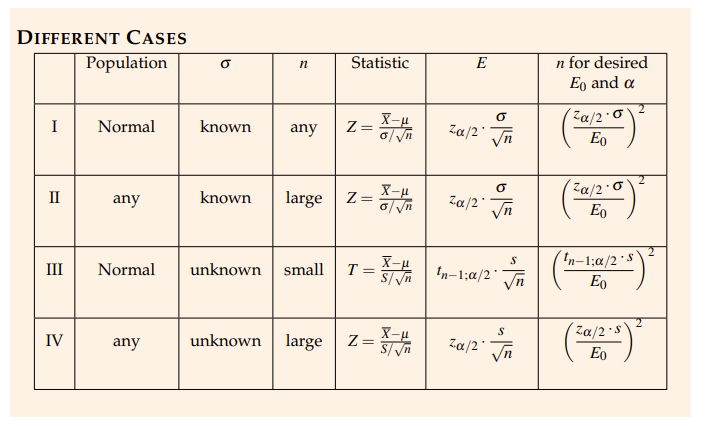
\includegraphics[width=1\linewidth]{cases.png}
\end{center}

\textbf{Confidence Interval} For confidence level $(1-\alpha)$, $P(a < \mu < b)=1-\alpha$, and $(a, b)$ is the confidence interval

\begin{center}
    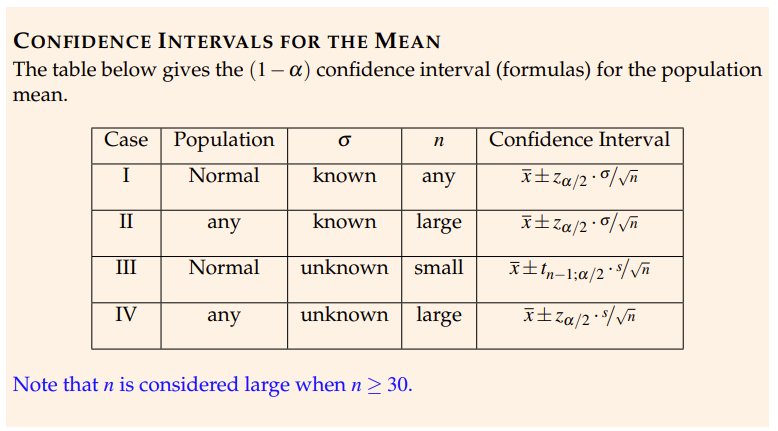
\includegraphics[width=1\linewidth]{intervals.png}
\end{center}

\textbf{Independent Samples} Complete randomisation

\textbf{Matched Pair Samples} Randomisation between matched pairs

\textbf{Independent Samples: Known, Unequal Variances}
\begin{enumerate}
    \item Random sample of size $n_1/n_2$ from population $1/2$ with mean $\mu_1/\mu_2$ and variance $\sigma_1^2/\sigma_2^2$
    \item The samples are independent
    \item The population variances are known and unequal
    \item Either both populations are normal or both samples are large
    \item $E(\overline{X}-\overline{Y})=\mu_1-\mu_2=\delta$
    \item $V(\overline{X}-\overline{Y})=\frac{\sigma_1^2}{n_1}+\frac{\sigma_2^2}{n_2}$
    \item Then $Z=\frac{(\overline{X}-\overline{Y})-(\mu_1-\mu_2)}{\sqrt{\frac{\sigma_1^2}{n_1}+\frac{\sigma_2^2}{n_2}}}$
    \item The $100(1-\alpha)\%$ confidence interval for $\mu_1-\mu_2$ is $(\overline{x}-\overline{y})\pm z_{\alpha/2}\sqrt{\frac{\sigma_1^2}{n_1}+\frac{\sigma_2^2}{n_2}}$
\end{enumerate}

\textbf{Independent Samples: Large, Unknown Variances}
\begin{enumerate}
    \item Random sample of size $n_1/n_2$ from population $1/2$ with mean $\mu_1/\mu_2$ and variance $\sigma_1^2/\sigma_2^2$
    \item The samples are independent
    \item The population variances are unknown and unequal
    \item Both samples are large
    \item The $100(1-\alpha)\%$ confidence interval for $\mu_1-\mu_2$ is $(\overline{X}-\overline{Y})\pm z_{\alpha/2}\sqrt{\frac{S_1^2}{n_1}+\frac{S_2^2}{n_2}}$
\end{enumerate}

\textbf{Independent Samples: Small, Equal Variances}
\begin{enumerate}
    \item Random sample of size $n_1/n_2$ from population $1/2$ with mean $\mu_1/\mu_2$ and variance $\sigma_1^2/\sigma_2^2$
    \item The samples are independent
    \item The population variances are unknown and the same
    \item Both samples are small
    \item Both populations are normally distributed
    \item $\sigma^2$ can be estimated by the pooled sample variance $S_p^2=\frac{(n_1-1)S_1^2+(n_2-1)S_2^2}{n_1+n_2-2}$
    \item $T=\frac{(\overline{X}-\overline{Y})-(\mu_1-\mu_2)}{S_p\sqrt{\frac{1}{n_1}+\frac{1}{n_2}}}\sim t_{n_1+n_2-2}$
    \item The $100(1-\alpha)\%$ confidence interval for $\mu_1-\mu_2$ is $(\overline{X}-\overline{Y})\pm t_{n_1+n_2-2;\alpha/2}S_p\sqrt{\frac{1}{n_1}+\frac{1}{n_2}}$
\end{enumerate}

\textbf{Independent Samples: Large, Equal Variances}
\begin{enumerate}
    \item Replace $t_{n_1+n_2-2;\alpha/2}$ with $z_{\alpha/2}$ in the previous formula
    \item The $100(1-\alpha)\%$ confidence interval for $\mu_1-\mu_2$ is $(\overline{X}-\overline{Y})\pm z_{\alpha/2}S_p\sqrt{\frac{1}{n_1}+\frac{1}{n_2}}$
    \item Equal Variance can be assumed if $0.5 \leq S_1/S_2 \leq 2$
\end{enumerate}

\textbf{Paired Data}
\begin{enumerate}
    \item $(X_1, Y_1),...,(X_n,Y_n)$ are matched pairs where $X_i/Y_i$ is a random sample from population $1/2$
    \item $X_i$ and $Y_i$ are dependent
    \item $(X_i,Y_i)$ and $(X_j,Y_j)$ are independent for $i\neq j$
    \item For matched pairs define $D_i=X_i-Y_i, \mu_D=\mu_1-\mu_2$
    \item We can treat $D_1,...,D_n$ as a random sample from a single population with mean $\mu_D$ and variance $\sigma_D^2$
    \item Consider $T=\frac{\overline{D}-\mu_D}{S_D / \sqrt{n}}$
    \item For small samples, if the population is normally distributed then $T\sim t_{n-1}$ and the confidence interval for $\mu_D$ is $\overline{d}\pm t_{n-1;\alpha/2}\cdot \frac{s_D}{\sqrt{n}}$
    \item For large samples then $T\sim N(0, 1)$ and the confidence interval for $\mu_D$ is $\overline{d}\pm z_{\alpha/2}\cdot \frac{s_D}{\sqrt{n}}$
\end{enumerate}

\section{Hypothesis Tests}
\textbf{How?}
\begin{enumerate}
    \item Set null and alternative hypotheses
    \item Set level of significance
    \item Identify test statistic, distribution, and rejection criteria
    \item Compute observed test statistic value
    \item Conclude
\end{enumerate}

\textbf{Null v/s Alternative Hypotheses}
We adopt the position of the null hypothesis unless there is overwhelming evidence against it. The hypothesis to be proven is the alternative hypothesis which often states the null hypothesis is false.

\textbf{Type I/II Errors}
Type I: Rejecting $H_0$ when $H_0$ is true, Type II: Not rejecting $H_0$ when $H_0$ is false.

\textbf{Level of Significance / Power}
Level of Significance: $\alpha=P(\text{Type I Error})$, Power: $1-\beta=P(\text{Reject $H_0$ | $H_0$ is False})$ where $\beta=P(\text{Type II Error})$

\textbf{Hypothesis Test for Mean: Known Variance}
\begin{enumerate}
    \item The population variance $\sigma^2$ is known and the underlying distribution is normal or sufficiently large
    \item For $H_0:\mu=\mu_0$, $Z=\frac{\overline{X}-\mu_0}{\sigma/\sqrt{n}}\sim N(0,1)$
    \item Let $z$ be the observed $Z$ value, then for the alternative hypothesis
    \item $H_1:\mu\neq\mu_0$, rejection region: $z<-z_{\alpha/2}$ or $z>z_{\alpha/2}$
    \item $H_1:\mu<\mu_0$, rejection region: $z<-z_\alpha$
    \item $H_1:\mu>\mu_0$, rejection region: $z>z_\alpha$
\end{enumerate}

\textbf{p-value}
\begin{itemize}
    \item Probability of obtaining a test statistic at least as extreme as the observed sample value given $H_0$ is true, a.k.a observed level of significance
    \item For 2 sided: $P(|Z|>|z|)=2P(Z>|z|)=2P(Z<-|z|)$
    \item 1 sided: $P(Z<-|z|)$ or $P(Z>|z|)$
    \item If p-value $< \alpha$, reject $H_0$, if not do not reject $H_0$
\end{itemize}

\textbf{Hypothesis test for Mean: Unknown Variance}
\begin{enumerate}
    \item The population variance $\sigma^2$ is unknown and the underlying distribution is normal
    \item For $H_0:\mu=\mu_0$, $T=\frac{\overline{X}-\mu_0}{S/\sqrt{n}}\sim t_{n-1}$
    \item Let $t$ be the observed $T$ value, then for the alternative hypothesis
    \item $H_1:\mu\neq\mu_0$, rejection region: $t<-t_{n-1;\alpha/2}$ or $t>t_{n-1;\alpha/2}$
    \item $H_1:\mu<\mu_0$, rejection region: $t<-t_{n-1;\alpha}$
    \item $H_1:\mu>\mu_0$, rejection region: $t>t_{n-1;\alpha}$
    \item When $n$ is large, $t_{n-1}$ can be replaced by $Z$
\end{enumerate}

\textbf{Comparing Means: Independent Samples I}
\begin{enumerate}
    \item The population variances $\sigma_1^2,\sigma_2^2$ are known and the underlying distributions are normal or samples are sufficiently large
    \item For $H_0:\mu_1-\mu_2=\delta_0$, $Z=\frac{(\overline{X}-\overline{Y})-\delta_0}{\sqrt{\frac{\sigma_1^2}{n_1}+\frac{\sigma_2^2}{n_2}}}\sim N(0,1)$
    \item When population variances are unknown and samples are sufficiently large
    \item For $H_0:\mu_1-\mu_2=\delta_0$, $Z=\frac{(\overline{X}-\overline{Y})-\delta_0}{\sqrt{\frac{S_1^2}{n_1}+\frac{S_2^2}{n_2}}}\sim N(0,1)$
\end{enumerate}
\begin{center}
    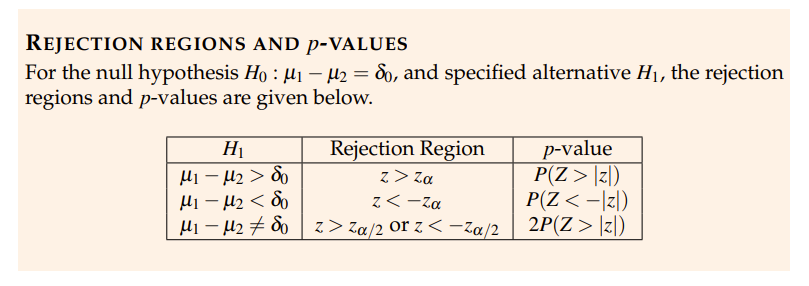
\includegraphics[width=\linewidth]{rejection.png}
\end{center}

\textbf{Comparing Means: Independent Samples II}
\begin{enumerate}
    \item The population variances $\sigma_1^2, \sigma_2^2$ are unknown but equal and the underlying distributions are normal and the samples are small
    \item For $H_0:\mu_1-\mu_2=\delta_0$, $Z=\frac{(\overline{X}-\overline{Y})-\delta_0}{S_p\sqrt{\frac{1}{n_1}+\frac{1}{n_2}}}\sim t_{n_1+n_2-2}$
\end{enumerate}

\begin{center}
\renewcommand{\arraystretch}{1.8}
\small
\begin{tabular}{|l|l|l|}
\hline
\textbf{Alt ($H_1$)} & \textbf{Reject $H_0$ if...} & \textbf{p-value} \\ \hline
$\mu_1 - \mu_2 > \delta_0$ & $T > t_{\alpha, \nu}$ & $P(T_{obs} > T)$ \\ \hline
$\mu_1 - \mu_2 < \delta_0$ & $T < -t_{\alpha, \nu}$ & $P(T_{obs} < T)$ \\ \hline
$\mu_1 - \mu_2 \neq \delta_0$ & $T > t_{\alpha/2, \nu}$ or $T < -t_{\alpha/2, \nu}$ & $2P(T_{obs} > |T|)$ \\ \hline
\end{tabular}
\end{center}

\textbf{Comparing Means: Paired Data}
\begin{enumerate}
    \item For paired data, $D_i=X_i-Y_i$
    \item For $H_0:\mu_D=\mu_{D_0}$, $T=\frac{\overline{D}-\mu_{D_0}}{S_D/\sqrt{n}}$
    \item If the sample is small and population is normally distributed then $T\sim t_{n-1}$
    \item If the sample is large then $T \sim N(0, 1)$
\end{enumerate}

\begin{center}
\renewcommand{\arraystretch}{1.8}
\small
\begin{tabular}{|l|l|l|}
\hline
\textbf{Alt ($H_1$)} & \textbf{Reject $H_0$ if...} & \textbf{p-value} \\ \hline
$\mu_D > \mu_{D_0}$ & $T > t_{\alpha, n-1}$ & $P(T_{obs} > T)$ \\ \hline
$\mu_D < \mu_{D_0}$ & $T < -t_{\alpha, n-1}$ & $P(T_{obs} < T)$ \\ \hline
$\mu_D \neq \mu_{D_0}$ & $T > t_{\alpha/2, n-1}$ or $T < -t_{\alpha/2, n-1}$ & $2 \times P(T_{obs} > |T|)$ \\ \hline
\end{tabular}
\end{center}

\end{multicols*}

\end{document}